\section{Introduction}
The purpose of this project is to analyze the stability (via Poincare map) of three simple running models to get a better understanding to the source of stability and robustness for fast runners. The three simple runners are:
	\begin{itemize}
	\item 2 DOF (Vertical) Hopper with pitch angle control
	\item Spring Loaded Inverted Pendulum (SLIP) model
	\item SLIP with Pendulum Runner (SLIPPER)
	\end{itemize}


\subsection{About the systems}
In this analysis, all the models are 2D runners.
The following are important common assumptions applied to all simple running models in this project
	\begin{itemize}
	\item The (steady-state) running motion is periodic.
	\item Massless leg -- No impact will be induced during foot collision.
	\item Energy conservation (especially for passive runners)
	\item Open-loop control on leg (e.g. open-loop leg force, or fixed touch-down angle for SLIP-based runners)
	\item Closed-loop control on pitch angle
	\end{itemize}
 
 \noindent Important parameters or quantities

\begin{itemize}
	\item Spring stiffness
	\item Running speed/running period/running frequency
	\item Duty factor $= \frac{t_{stance}}{t_{stance}+t_{flight}}$	
	\item Fast running index (proposed by IHMC)
\end{itemize}

 \noindent Other important concepts (of fast runner)
\begin{itemize}
	\item Meta center
	\item Resonance -- Please check Jorge Cham's thesis \cite{Cham2002} 2.2 Resonance in Running.
	\item Please refer to fast runner meeting notes or proposal for more information.
\end{itemize}

\subsection{Related research}
\begin{itemize}
	\item Jorge Cham's Dissertation \cite{Cham2002}
	\item David Remy's Dissertation \cite{Remy2011}
	\item Shen's paper about SLIP model analysis \cite{Shen2016}
\end{itemize}

\subsection{About the method of stability analysis used in this project}
\textbf{Some "must-have" and "nice-to-have" requirements for the analysis method}
\begin{itemize}
\item Stability analysis
\item Robustness
\item Dimension analysis (so that it can be used for robots with different scales)
\item Applicable to complex system (e.g. for the designed mechanism)
\end{itemize}

For the requirements listed above, and also to explore the nonlinearity and coupled dynamics for SLIP-based runners, the main method for stability analysis used in this project contains two parts:
\begin{itemize}
	\item Trajectory optimization using single-shooting method -- For finding periodic motions.
	\item Poincare Map -- Check the Eigen values of the Poincare map (it is a matrix) of a periodic motion to determine its stability.
\end{itemize}

\noindent Please refer to
\href{https://confluence.ihmc.us/display/FR/Description+of+how+to+find+limit+cycles+and+Poincare+maps+from+Andy+Ruina}{Description of how to find limit cycles and Poincare maps from Andy Ruina}, the note has great numerical recipe for better Poincare map approximation and stability analysis.

\subsubsection{About the Poincare section and Poincare map}
Please check Jorge Cham's thesis \cite{Cham2002} Chapter 2 for more information.
\subsubsection{About the Trajectory optimization using single shooting method}
This method is widely used for finding stable limit cycles for passive walkers. For more imformation, please check \href{http://www.matthewpeterkelly.com/tutorials/trajectoryOptimization/canon.html}{Matthew Kelly's web page about Canon examples using different trajectory optimization methods}.
\subsection{Fast running index}
Please refer to fast runner meeting notes or proposal for more information.
\subsection{Other links}
\begin{itemize}
	\item \href{https://confluence.ihmc.us/x/Q4BIC}{Ken's slides on the Confluence page}
	\item project Repo: \href{https://stash.ihmc.us/projects/ICSL/repos/fast-runner-analysis}{https://stash.ihmc.us/projects/ICSL/repos/fast-runner-analysis}
	\item SCS implementation: RoundRunner under Fast Runner: \href{https://stash.ihmc.us/projects/ICSL/repos/fast-runner/browse/fast-runner/src/main/java/us/ihmc/fastRunner/RoundRunner}{https://stash.ihmc.us/projects/ICSL/repos/fast-runner/browse/fast-runner/src/main/java/us/ihmc/fastRunner/RoundRunner}
\end{itemize}

%\subsection{Remarks}
%\begin{itemize}
%\item Impact does not cause velocity change on runner with massless leg!
%\item In SCS, to simulate massless leg, it is better to use only one body, and manipulate the relation between the contact point and the body in controller instead.
%\end{itemize}

%\subsection{Questions}
%About Directions
%\begin{itemize}
%\item Should I exclude the gyroscopic-based stabilization? 
%\item The linkage between the control in simulation and mechanism design
%	\begin{itemize}
%	\item Parameters
%	\item How to design a mechanism can emulate PD control?
%	\end{itemize}
%\end{itemize}
%General Utilities 
%\begin{itemize}
%\item Any solver for nonlinear program IHMC used?
%\item Any trajectory optimization package IHMC used?
%\item Methods to get stable Reciprocating Spoked Runner?
%\end{itemize}
%
%Past simulations
%\begin{itemize}
%\item Why the abstract runner (in spoked runner project) can be stabilized in x direction? 
%\begin{figure}[h]
%\centering
%
%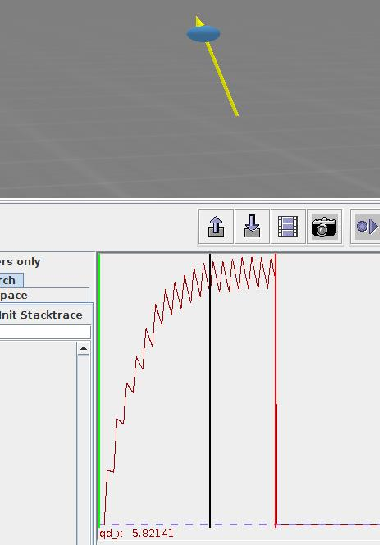
\includegraphics[scale = 0.5]{abstractRunner.pdf} 
%\caption{The Abstract Runner}
%%\label{fig.1DOF-Hopper}
%\end{figure}
%\begin{itemize}
%\item The simulation setup is really robust for a large set of initial conditions/throttle angles
%\item It turns out its because the added \underline{wind resistance} dissipate a lot of energies.
%\end{itemize}
%
%
%\item Methods to get stable Reciprocating Spoked Runner?
%\item What is the line \underline{private static final long serialVersionUID } for?
%
%\end{itemize}

\pagebreak